\begin{figure}[b!]
  \centering
  \begin{subfigure}[t]{0.48\linewidth}
    \centering
    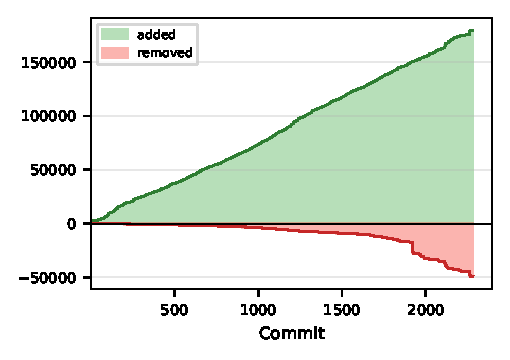
\includegraphics[width=\linewidth]{images/churn_over_time_by_commit.pdf}
    \subcaption{\small Added and removed lines}
    \label{fig:churn}
  \end{subfigure}\hfill
  \begin{subfigure}[t]{0.48\linewidth}
    \centering
    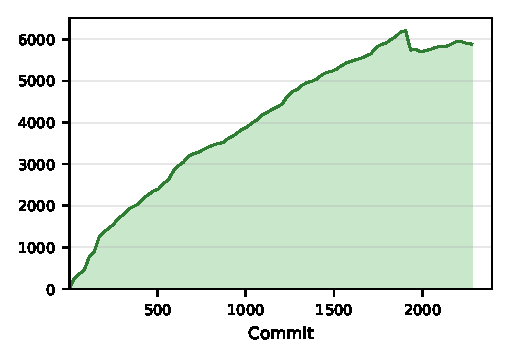
\includegraphics[width=\linewidth]{images/declarations_over_time_by_commit.pdf}
    \subcaption{\small Lean declarations}
    \label{fig:decls}
  \end{subfigure}
  \caption{\textbf{Progress of the automatic formalization system.} Two phases are clearly discernible: continuous code base expansion (including unnecessary \emph{rabbit hole} content) and cleanup triggered by an update in agent prompts. Each commit represents a separate agent that merges its work into the main branch. At the end, all 340 \emph{target theorems} and definitions are present and proved.}
  \label{fig:churn-decls}
\end{figure}
